\documentclass[11pt, a4paper, twocolumn]{article}
\usepackage[a4paper,margin=1in,footskip=0.25in]{geometry}
 
\usepackage{graphicx}
\usepackage{enumerate}
\usepackage[utf8]{inputenc}
\usepackage{xcolor}
\usepackage{hyperref}
\usepackage{subfig}
\usepackage{floatrow}

\usepackage{amsmath}
\usepackage{amssymb}
\usepackage{arydshln}

\usepackage{tikz}
\usetikzlibrary{positioning,arrows,decorations.markings}

\newcommand{\tjzm}{$t$-$J^z$~model}
\newcommand{\ket}[1]{\left\vert #1 \right\rangle}
\newcommand{\bra}[1]{\left\langle #1 \right\vert}
\newcommand{\abs}[1]{\left\vert #1 \right\vert}

\def\K{%
    \operatornamewithlimits{%
        \mathchoice{% * Display style
            \vcenter{\hbox{\huge $\mathcal{K}$}}%
        }{%           * Text style
            \vcenter{\hbox{\Large $\mathcal{K}$}}%
        }{%           * Script style
            \mathrm{\mathcal{K}}%
        }{%           * Script script style
            \mathrm{\mathcal{K}}%
        }
    }
}

\def\composition{\operatornamewithlimits{\circ}}

\providecommand{\newoperator}[3]{%
	\newcommand*{#1}{\mathop{#2}#3}}
\providecommand{\renewoperator}[3]{%
	\renewcommand*{#1}{\mathop{#2}#3}}
	
\newoperator{\srot}%
	{\mathrm{rot}}{\nolimits}

\newoperator{\ent}%
	{\mathrm{ent}}{\nolimits}
	
\renewoperator{\Re}%
	{\mathrm{Re}}{\nolimits}
	
\renewoperator{\Im}%
	{\mathrm{Im}}{\nolimits}	
	
\makeatletter
\providecommand*{\diff}%
	{\@ifnextchar^{\DIfF}{\DIfF^{}}}
	
\def\DIfF^#1{%
	\mathop{\mathrm{\mathstrut d}}%
	\nolimits^{#1}\gobblespace}
	
\def\gobblespace{%
	\futurelet\diffarg\opspace}
	
\def\opspace{%
	\let\DiffSpace\!%
		\ifx\diffarg(%
			\let\DiffSpace\relax
		\else
			\ifx\diffarg[%
				\let\DiffSpace\relax
			\else
				\ifx\diffarg\{%
					\let\DiffSpace\relax
				\fi\fi\fi\DiffSpace}
				
\providecommand*{\deriv}[3][]{%
	\frac{\diff^{#1}#2}{\diff #3^{#1}}}
\providecommand*{\pderiv}[3][]{%
	\frac{\partial^{#1}#2}%
		{\partial #3^{#1}}}
		
\newcommand{\mean}[1]{\langle#1\rangle}

\begin{document}

\section{Method}
Local Greens function with rotational degrees of freedom can be written as
\begin{equation}
    G^{\text{rot}}_{M_n}(\omega) = 
    \bra{0_\sigma}R^{\dag}_{\sigma,M_n}(0) 
        \hat{G}(\omega)
    R_{\sigma,M_n}(0) \ket{0_\sigma}.
\end{equation}
where $\hat{G}(\omega) = (\omega - H + E_0)^{-1}$.  $H = \mathcal{H}_t + \mathcal{H}_J$ stands for the \tjzm{} Hamiltonian with the ground state $\ket{0_\sigma}$ in the half-filled limit. We denote energy of $\ket{0_\sigma}$ as $E_0$. The label $\sigma \in \{-1/2, 1/2\}$ stands for the spin at the origin of the lattice, i.e. at site $i = 0$. Operator $R_{\sigma,M_n}(i)$ removes the electon with spin $\sigma$ from site $i$ and then creates a normalised linear combination of states where the created hole has been propagated exactly $n$ times without returning. With each hop the hole acquires a phase proportional to $M_n(j) = m^{(j)}$, where $M_n = (m^{(1)}, ..., m^{(n)})$ is ordered collection of phase factors.

Within the self-avoiding walks approximation operator $R_{\sigma,M_n}(i)$ is restricted only to paths that do not cross themselves. In the same time, the rotational Greens function can be rewritten in the following form,
\begin{equation}
    G^{\text{rot}}_{M_n}(\omega) = 
    \frac{1}{\abs{\mathcal{A}_n}}\sum_{\eta, \eta' \in \mathcal{A}_n}
	\mathcal{P}_{M_n}^{\eta',\eta}
        %e^{i m(\varphi_\xi - \varphi_{\xi'})}
        G_{\eta', \eta}(\omega),
\end{equation}
where $\ket{\eta}$ and $\ket{\eta'}$ denote states with the hole created at the origin $(i = 0)$ and propagated $n$ times to site $j \neq 0$, such that the hole does not cross its own path. We call this type of the motion of the hole a self-avoiding walk (or self-avoiding path) and denote the set of self-avoiding paths with length $n$ as $\mathcal{A}_n$. We also define the coefficient of the Greens function,
\begin{equation}
    G_{\eta', \eta}(\omega) = \bra{\eta'}\hat{G}(\omega)\ket{\eta},
\end{equation}
and the phase contribution from the angular momentum of the hole is denoted as $\mathcal{P}_{M_n}^{\eta',\eta}$. 

Calculation of the phases is a trivial. For an example have a look at the appendix (...). 

The task is to calculate coeffcient $G_{\eta', \eta}(\omega)$ for a given pair of self-avoiding paths $\eta$ and $\eta'$.
Let us denote $\hat{H}(\omega) = (\omega - H + E_0)$ such that $\hat{G}(\omega) = \hat{H}(\omega)^{-1}$. Then let define basis $\mathcal{B}$ of all possible states $\ket{\eta}$ of the system, where there exists $n$ such that $\eta \in \mathcal{A}_n$. In general we can find elements $G_{\eta', \eta}(\omega)$ with cofactor matrix method,
\begin{equation}
    \mathcal{M}(\hat{G}(\omega))_\mathcal{B}^\mathcal{B} = 
    \frac{C^{T}(\omega)}{\det \mathcal{M}(\hat{H}(\omega))_\mathcal{B}^\mathcal{B}},
\end{equation}
where matrix $C = [C_{i,j}]$, coefficients $C_{i,j} = (-1)^{i+j}M_{i,j}$ and $M_{i,j}$ is the $(i,j)$-minor of the matrix $\mathcal{M}(\hat{H}(\omega))_\mathcal{B}^\mathcal{B}$ with $i$-th row and $j$-th column removed. 

Let $\eta_n = \xi_1 \xi_2 \hdots \xi_n$ for $n>0$, where $\xi_j \in D$ denotes $j$-th move of the hole and $\eta_0 = 1$ for $n=0$. On a square lattice (or on the Bethe lattice) with coordination number $z=4$ we can put for example $D = \{E,N,W,S\}$ denoting 4 possible directions of the propagation from each site.

Let us further introduce function $\mathcal{S}$ that takes a self-avoiding path $\eta_n$ of the hole and returns set of moves $\Delta$ leading to the self-avoiding paths $\eta_{n+1} = \eta_n \xi_{n+1}$ reachable from the path $\eta_n$. Then we can write,
\begin{equation}\label{eq:Sigma}
    t^2\Sigma_{\eta_k}(\omega)^{-1} = G_{\eta_k}(\omega)^{-1} - \sum_{\xi \in \mathcal{S}(\eta_k)}\Sigma_{\eta_k \xi}(\omega),
\end{equation}
where
\begin{equation}
    G_{\eta_k}(\omega)^{-1} = 
    \bra{\eta_k}
    \left(
        \omega - \mathcal{H}_J + E_{0}
    \right)
    \ket{\eta_k}.
\end{equation}
Moreover we define,
\begin{equation}\label{eq:Gamma}
    \Gamma_{\eta_k}^{\Delta}(\omega) = G_{\eta_k}(\omega)^{-1} - \sum_{\xi \in \Delta}\Sigma_{\eta_k \xi}(\omega),
\end{equation}
where $\Delta \subset D$. The above defined $\Gamma_\eta^{\Delta}(\omega)$ can be evalueted numerically assuming finite depth of the recursion in the Eq.~\eqref{eq:Sigma}. One can adjust the depth of the recursion to ensure convergence, provided that the value of the coupling constant is not too small, i.e. $J > 0.2t$ for the square lattice or $J > 0.01t$ for the Bethe lattice where symmetry allows for improvements.

In the end, the generic formula for $G_{\eta'_l, \eta_r}(\omega)$ can be found in the following form, 
\begin{equation}\label{eq:GFcoef}
	\begin{split}
		&\bra{\xi'_1 \xi'_2 \hdots \xi'_l}
		\hat{G}(\omega)
		\ket{\xi_1 \xi_2 \hdots \xi_r} = (-t)^{r + l - 2c} \times \\
		&\frac{\displaystyle
		\prod_{k=0}^{c-1} \left(
			\Gamma_{\eta_k}^{\mathcal{S}(\eta_k)\setminus\{\xi_{k+1}\}} - \K_{n=k+1}^{c-1} \frac{t^2}{\Gamma_{\eta_n}^{\mathcal{S}(\eta_n)\setminus\{\xi_{n+1}\}}}
		\right)
		}{\displaystyle
		\left(
			\prod_{k=0}^{c} \Gamma_{\eta_k}^{\mathcal{S}(\eta_k)}
		\right)
		\left(
			\prod_{k=c+1}^{r} \Gamma_{\eta_k}^{\mathcal{S}(\eta_k)}
		\right)
		\left(
			\prod_{k=c+1}^{l} \Gamma_{\eta_k}^{\mathcal{S}(\eta_k)}
		\right)
		},    
	\end{split}
\end{equation}
where we have $\xi'_j = \xi_j$ for all $j \leq c$ and either $c = \min(l,r)$ or $\xi'_{c+1} \neq \xi_{c+1}$. Moreover, to shorten the notation we write $\Gamma_\eta^\Delta \equiv \Gamma_\eta^\Delta(\omega)$.

To grasp the essence of the equation \eqref{eq:GFcoef} for $G_{\eta', \eta}(\omega)$ it is instructive to express it through diagrams. To this end, let us formulate rules for creating the diagrams in terms of the introduced notation. 
\begin{enumerate}
    \item Diagram consists of nodes connected with single lines or double lines. Nodes correspond to states of the system, while lines represent the propagation of the hole. Single lines represent propagation distinct in the left $\bra{\eta'}$ and the right $\ket{\eta}$ states while double lines correspond to common parts of the path.
    \item Each node is labeled with its corresponding weight $\Gamma_{\eta}^{\mathcal{S}(\eta)}$, where $\eta$ is state of the system in moves notation.
    \item Single lines are denoted with $-t$ as they add a factor of $-t$ to the whole solution.
    \item Double line corresponding to move $\xi \in D$ and starting from the node denoted with $\Gamma_{\eta}^{\mathcal{S}(\eta)}$ is denoted with $\Gamma_{\eta}^{\mathcal{S}(\eta) \setminus \{\xi\}}$.
    \item Each line ends with arrow denoting direction of hole motion (i.e. order of operators $\xi_j \in D$) in the left and the right state.
\end{enumerate}

With the above, the local Greens function can be written as follows,
\begin{equation}
    G_{1,1}(\omega) = \frac{1}{\Gamma_1^{D}(\omega)},
\end{equation}
or expressed through the simplest diagram.
\begin{center}
	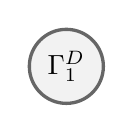
\begin{tikzpicture}[
	roundnode/.style={circle, draw=black!60, fill=black!5, very thick, minimum size=0.25}
	]
		%Nodes
		\node[roundnode]    
			(m0)                    {$\Gamma_1^{D}$};
			
	\end{tikzpicture} 
\end{center}
For the coefficient $G_{EE,EE}$ the diagram is as follows,
\begin{center}
    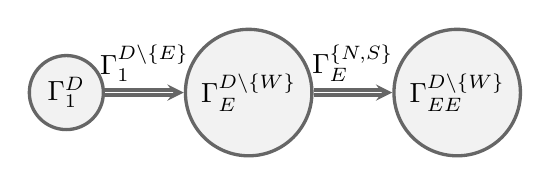
\begin{tikzpicture}[
    roundnode/.style={circle, draw=black!60, fill=black!5, very thick, minimum size=0.25}
    ]
        %Nodes
        \node[roundnode]    
            (m0)                    {$\Gamma_1^{D}$};
        \node[roundnode]    
            (mE)    [right=of m0]   {$\Gamma_E^{D \setminus \{W\}}$};
        \node[roundnode]    
            (mEE)    [right=of mE]   {$\Gamma_{EE}^{D \setminus \{W\}}$};
        
        %Lines
        \draw[->, >=stealth, draw=black!60, very thick, double] 
            (m0.east) -- node[above] {$\Gamma_1^{D \setminus \{E\}}$} (mE.west);
        \draw[->, >=stealth, draw=black!60, very thick, double] 
            (mE.east) -- node[above] {$\Gamma_E^{\{N,S\}}$} (mEE.west);
    \end{tikzpicture}
\end{center}
so we can read out the expression,
\begin{equation}
	G_{EE,EE}(\omega) = \frac{
	\left(
	\Gamma_1^{D \setminus \{E\}}
	-\frac{t^2}{\Gamma_E^{\{N,S\}}}
	\right)
	\Gamma_E^{\{N,S\}}
	}
	{
		\Gamma_1^{D}
		\Gamma_E^{D \setminus \{W\}}
		\Gamma_{EE}^{D \setminus \{W\}}
	}.
\end{equation}
Compare it with the Eq.~\eqref{eq:GFcoef}. Similarily for $G_{EN,EE}$,
\begin{center}
    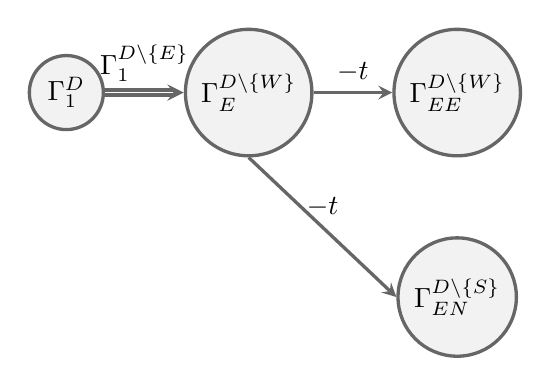
\begin{tikzpicture}[
    roundnode/.style={circle, draw=black!60, fill=black!5, very thick, minimum size=0.25}
    ]
        %Nodes
        \node[roundnode]    
            (m0)                    {$\Gamma_1^{D}$};
        \node[roundnode]    
            (mE)    [right=of m0]   {$\Gamma_E^{D \setminus \{W\}}$};
        \node[roundnode]    
            (mEE)    [right=of mE]   {$\Gamma_{EE}^{D \setminus \{W\}}$};
        \node[roundnode]    
            (mEN)    [below=of mEE]   {$\Gamma_{EN}^{D \setminus \{S\}}$};
        
        %Lines
        \draw[->, >=stealth, draw=black!60, very thick, double] 
            (m0.east) -- node[above] {$\Gamma_1^{D \setminus \{E\}}$} (mE.west);
        \draw[->, >=stealth, draw=black!60, very thick] 
            (mE.east) -- node[above] {$-t$} (mEE.west);
        \draw[->, >=stealth, draw=black!60, very thick] 
            (mE.south) -- node[above] {$-t$} (mEN.west);
    \end{tikzpicture}
\end{center}
we can read out the formula from its diagram,
\begin{equation}
	G_{EE,EN}(\omega) = \frac{
	t^2\Gamma_1^{D \setminus \{E\}}
	}
	{
		\Gamma_1^{D}
		\Gamma_E^{D \setminus \{W\}}
		\Gamma_{EE}^{D \setminus \{W\}}
		\Gamma_{EN}^{D \setminus \{S\}}
	}.
\end{equation}

Moreover, while performing the calculations one shall take the advantage of the symmetries of the system, e.g. $G_{EE,EE} = G_{NN,NN} = G_{WW,WW} = G_{SS,SS}$, to reduce the number of terms that have to be calculated to find Greens function with rotations.

\clearpage

\begin{figure*}[ht!]
	\includegraphics[width=0.49\columnwidth]
	{./figures/square/Int64[].png}
	\includegraphics[width=0.49\columnwidth]
	{./figures/bethe/Int64[].png}
	\caption{
		Spectral function $A(\omega)$ of a singe hole doped to the Ising antiferromagnet calculated within self-avoiding walks approximation (with interactions included), (a) on the square lattice and (b) on the Bethe lattice. Coupling constant $J=0.4t$.
	}
\end{figure*}

\begin{figure*}[ht!]
	\includegraphics[width=0.49\columnwidth]
	{./figures/square/[0].png}
	\includegraphics[width=0.49\columnwidth]
	{./figures/bethe/[0].png}
	\caption{
		Spectral function $A(\omega)$ of a singe hole with rotational degrees of freedom calculated within self-avoiding walks approximation (with interactions included), (a) on the square lattice and (b) on the Bethe lattice. Coupling constant $J=0.4t$, $m_4 = 0$.
	}
\end{figure*}

\begin{figure*}[ht!]
	\includegraphics[width=0.49\columnwidth]
	{./figures/square/[1].png}
	\includegraphics[width=0.49\columnwidth]
	{./figures/bethe/[1].png}
	\caption{
		Spectral function $A(\omega)$ of a singe hole with rotational degrees of freedom calculated within self-avoiding walks approximation (with interactions included), (a) on the square lattice and (b) on the Bethe lattice. Coupling constant $J=0.4t$, $m_4 = 1$.
	}
\end{figure*}

\clearpage

\begin{figure*}[ht!]
	\includegraphics[width=0.49\columnwidth]
	{./figures/square/[0, 0].png}
	\includegraphics[width=0.49\columnwidth]
	{./figures/bethe/[0, 0].png}
	\caption{
		Spectral function $A(\omega)$ of a singe hole with rotational degrees of freedom calculated within self-avoiding walks approximation (with interactions included), (a) on the square lattice and (b) on the Bethe lattice. Coupling constant $J=0.4t$, $m_4 = 0$, $m_3 = 0$.
	}
\end{figure*}

\begin{figure*}[ht!]
	\includegraphics[width=0.49\columnwidth]
	{./figures/square/[0, 1].png}
	\includegraphics[width=0.49\columnwidth]
	{./figures/bethe/[0, 1].png}
	\caption{
		Spectral function $A(\omega)$ of a singe hole with rotational degrees of freedom calculated within self-avoiding walks approximation (with interactions included), (a) on the square lattice and (b) on the Bethe lattice. Coupling constant $J=0.4t$, $m_4 = 0$, $m_3 = 1$.
	}
\end{figure*}

\begin{figure*}[ht!]
	\includegraphics[width=0.49\columnwidth]
	{./figures/square/[1, 0].png}
	\includegraphics[width=0.49\columnwidth]
	{./figures/bethe/[1, 0].png}
	\caption{
		Spectral function $A(\omega)$ of a singe hole with rotational degrees of freedom calculated within self-avoiding walks approximation (with interactions included), (a) on the square lattice and (b) on the Bethe lattice. Coupling constant $J=0.4t$, $m_4 = 1$, $m_3 = 0$.
	}
\end{figure*}

\begin{figure*}[ht!]
	\includegraphics[width=0.49\columnwidth]
	{./figures/square/[1, 1].png}
	\includegraphics[width=0.49\columnwidth]
	{./figures/bethe/[1, 1].png}
	\caption{
		Spectral function $A(\omega)$ of a singe hole with rotational degrees of freedom calculated within self-avoiding walks approximation (with interactions included), (a) on the square lattice and (b) on the Bethe lattice. Coupling constant $J=0.4t$, $m_4 = 1$, $m_3 = 1$.
	}
\end{figure*}

\clearpage

\begin{figure*}[ht!]
	\includegraphics[width=0.49\columnwidth]
	{./figures/square/Int64[]_noint.png}
	\includegraphics[width=0.49\columnwidth]
	{./figures/bethe/Int64[]_noint.png}
	\caption{
		Spectral function $A(\omega)$ of a singe hole doped to the Ising antiferromagnet calculated within self-avoiding walks approximation without interactions, (a) on the square lattice and (b) on the Bethe lattice. Coupling constant $J=0.4t$.
	}
\end{figure*}

\begin{figure*}[ht!]
	\includegraphics[width=0.49\columnwidth]
	{./figures/square/[0]_noint.png}
	\includegraphics[width=0.49\columnwidth]
	{./figures/bethe/[0]_noint.png}
	\caption{
		Spectral function $A(\omega)$ of a singe hole with rotational degrees of freedom calculated within self-avoiding walks approximation without interactions, (a) on the square lattice and (b) on the Bethe lattice. Coupling constant $J=0.4t$, $m_4 = 0$.
	}
\end{figure*}

\begin{figure*}[ht!]
	\includegraphics[width=0.49\columnwidth]
	{./figures/square/[1]_noint.png}
	\includegraphics[width=0.49\columnwidth]
	{./figures/bethe/[1]_noint.png}
	\caption{
		Spectral function $A(\omega)$ of a singe hole with rotational degrees of freedom calculated within self-avoiding walks approximation without interactions, (a) on the square lattice and (b) on the Bethe lattice. Coupling constant $J=0.4t$, $m_4 = 1$.
	}
\end{figure*}

\clearpage

\begin{figure*}[ht!]
	\includegraphics[width=0.49\columnwidth]
	{./figures/square/[0, 0]_noint.png}
	\includegraphics[width=0.49\columnwidth]
	{./figures/bethe/[0, 0]_noint.png}
	\caption{
		Spectral function $A(\omega)$ of a singe hole with rotational degrees of freedom calculated within self-avoiding walks approximation without interactions, (a) on the square lattice and (b) on the Bethe lattice. Coupling constant $J=0.4t$, $m_4 = 0$, $m_3 = 0$.
	}
\end{figure*}

\begin{figure*}[ht!]
	\includegraphics[width=0.49\columnwidth]
	{./figures/square/[0, 1]_noint.png}
	\includegraphics[width=0.49\columnwidth]
	{./figures/bethe/[0, 1]_noint.png}
	\caption{
		Spectral function $A(\omega)$ of a singe hole with rotational degrees of freedom calculated within self-avoiding walks approximation without interactions, (a) on the square lattice and (b) on the Bethe lattice. Coupling constant $J=0.4t$, $m_4 = 0$, $m_3 = 1$.
	}
\end{figure*}

\begin{figure*}[ht!]
	\includegraphics[width=0.49\columnwidth]
	{./figures/square/[1, 0]_noint.png}
	\includegraphics[width=0.49\columnwidth]
	{./figures/bethe/[1, 0]_noint.png}
	\caption{
		Spectral function $A(\omega)$ of a singe hole with rotational degrees of freedom calculated within self-avoiding walks approximation without interactions, (a) on the square lattice and (b) on the Bethe lattice. Coupling constant $J=0.4t$, $m_4 = 1$, $m_3 = 0$.
	}
\end{figure*}

\begin{figure*}[ht!]
	\includegraphics[width=0.49\columnwidth]
	{./figures/square/[1, 1]_noint.png}
	\includegraphics[width=0.49\columnwidth]
	{./figures/bethe/[1, 1]_noint.png}
	\caption{
		Spectral function $A(\omega)$ of a singe hole with rotational degrees of freedom calculated within self-avoiding walks approximation without interactions, (a) on the square lattice and (b) on the Bethe lattice. Coupling constant $J=0.4t$, $m_4 = 1$, $m_3 = 1$.
	}
\end{figure*}

\clearpage

\newpage

\section*{Acknowledgements}
We  kindly  acknowledge  support  by  the  (Polish)  National  Science  Centre  (NCN, Poland)  under  Projects  No. 2016/22/E/ST3/00560 (PW and KW), 2016/23/B/ST3/00839 (KW). The calculations were performed at the ICM cluster.


\end{document}